% This is the Reed College LaTeX thesis template. Most of the work
% for the document class was done by Sam Noble (SN), as well as this
% template. Later comments etc. by Ben Salzberg (BTS). Additional
% restructuring and APA support by Jess Youngberg (JY).
% Your comments and suggestions are more than welcome; please email
% them to cus@reed.edu
%
% See http://web.reed.edu/cis/help/latex.html for help. There are a
% great bunch of help pages there, with notes on
% getting started, bibtex, etc. Go there and read it if you're not
% already familiar with LaTeX.
%
% Any line that starts with a percent symbol is a comment.
% They won't show up in the document, and are useful for notes
% to yourself and explaining commands.
% Commenting also removes a line from the document;
% very handy for troubleshooting problems. -BTS

% As far as I know, this follows the requirements laid out in
% the 2002-2003 Senior Handbook. Ask a librarian to check the
% document before binding. -SN

%%
%% Preamble
%%
% \documentclass{<something>} must begin each LaTeX document
\documentclass[12pt,twoside,openany]{reedthesis}
% Packages are extensions to the basic LaTeX functions. Whatever you
% want to typeset, there is probably a package out there for it.
% Chemistry (chemtex), screenplays, you name it.
% Check out CTAN to see: http://www.ctan.org/
%%

\usepackage{setspace}
\usepackage{graphicx,latexsym}
\usepackage{amsmath}
\usepackage{amssymb,amsthm}
\usepackage{longtable,booktabs,setspace, array}
\usepackage[hyphens]{url}
\usepackage{hyperref}
% Added by JLB
\usepackage{lineno} % line numbers
\linenumbers

\usepackage{lmodern}

\usepackage{float}
\floatplacement{figure}{h}

\usepackage{rotating}

\usepackage{natbib}
% Comment out the natbib line above and uncomment the following two lines to use the new
% biblatex-chicago style, for Chicago A. Also make some changes at the end where the
% bibliography is included.
% \usepackage{biblatex-chicago}
% \bibliography{thesis}


% Added by CII (Thanks, Hadley!)
% Use ref for internal links
\renewcommand{\hyperref}[2][???]{\autoref{#1}}
\def\chapterautorefname{Chapter}
\def\sectionautorefname{Section}
\def\subsectionautorefname{Subsection}
% End of CII addition

% Added by CII
\usepackage{caption}
\captionsetup{width=5in}
% End of CII addition

% \usepackage{times} % other fonts are available like times, bookman, charter, palatino

% Syntax highlighting #22

% To pass between YAML and LaTeX the dollar signs are added by CII
\title{Regime Detection Measures for the Practical Ecologist}
\author{Jessica L. Burnett}
% The month and year that you submit your FINAL draft TO THE LIBRARY
\date{2019}
% \division{}
\advisor{Craig R. Allen}
\department{School of Natural Resources}
\institution{University of Nebraska-Lincoln}
\degree{Doctor of Philosophy}
%If you have two advisors for some reason, you can use the following
% Uncommented out by CII
\altadvisor{Dirac Twidwell}
% End of CII addition

%%% Remember to use the correct department!
% if you're writing a thesis in an interdisciplinary major,
% uncomment the line below and change the text as appropriate.
% check the Senior Handbook if unsure.
%\thedivisionof{The Established Interdisciplinary Committee for}
% if you want the approval page to say "Approved for the Committee",
% uncomment the next line
%\approvedforthe{Committee}

% Added by CII
%%% Copied from knitr
%% maxwidth is the original width if it's less than linewidth
%% otherwise use linewidth (to make sure the graphics do not exceed the margin)
\makeatletter
\def\maxwidth{ %
  \ifdim\Gin@nat@width>\linewidth
    \linewidth
  \else
    \Gin@nat@width
  \fi
}
\makeatother

\renewcommand{\contentsname}{Table of Contents}
% End of CII addition

\setlength{\parskip}{0pt}

% Added by CII

\providecommand{\tightlist}{%
  \setlength{\itemsep}{0pt}\setlength{\parskip}{0pt}}

\Acknowledgements{

}

\Dedication{

}

\Preface{

}

\Abstract{

}

% End of CII addition
%%
%% End Preamble
%%
%
\begin{document}

% Everything below added by CII
  \maketitle

\frontmatter % this stuff will be roman-numbered
\pagestyle{empty} % this removes page numbers from the frontmatter

%

  \hypersetup{linkcolor=black}
  \setcounter{tocdepth}{2}
  \tableofcontents

  \listoftables

  \listoffigures


%
\mainmatter % here the regular arabic numbering starts
\pagestyle{fancyplain} % turns page numbering back on
\doublespacing{} % Trying to set spacing between lines in body
% \linespread{1.6} % Trying to set spacing between lines in body

\chapter{thesisdown::thesis\_gitbook:
default}\label{thesisdownthesis_gitbook-default}

Placeholder

Identifying abrupt changes in the structure and functioning of systems,
or system regime shifts, in ecological and social-ecological systems
leads to an understanding of relative and absolute system resilience.
Resilience is an emergent phenomenon of complex social-ecological
systems, and is the ability of a system to absorb disturbance without
reorganizing into a new state, or regime. Resilience science provides a
framework and methodology for quantitatively assessing the capacity of a
system to maintain its current trajectory (or to stay within a certain,
and often desirable regime). If and when a system's resilience is
exceeded, it crosses a threshold and enters into an alternate regime (or
undergoes a regime shift).\\
I will use Fisher Information to detect regime shifts in time and space
using avian community data obtained from the North American Breeding
Bird Survey within the area east of the Rockies and west of the
Mississippi River. Fisher Information is a technique that captures the
dynamic of a system, and this metric will be calculated about a suite of
bird species abundances aggregated to the route level for all possible
time periods. Transmutation (aggregation error) about inclusion or
exclusion of certain bird species, functional groups, and guilds will be
analyzed. Efforts have been made to develop early warning indicators of
regime shifts in ecosystems, however, for most ecosystems there is great
uncertainty in predicting the risk of a regime shift, regarding both
when and how long it will take to happen and if it can be recognized
early enough to be avoided when desired. We will complement the use of
Fisher Information with multiple discontinuity analyses about body mass
distributions at the route-level to achieve the aim of identifying
individual species that best serve as early-warning indicators of regime
shifts. For those species found on the edges of body mass aggregations,
we test the hypothesis that the background variance in their abundances
(on Breeding Bird Survey routes) will increase more than those not
observed at the edge of discontinuity aggregations. Identification of
early-warning indicators of regime shifts in ecological systems allows
management efforts to focus on a single or a small number of species
that inform us about ecosystem resilience and trajectory.\\
These methods transcend the primary objective of the Breeding Bird
Survey (to monitor population trends) and use this expansive dataset in
such a way that information about ecosystem order, trajectory, and
resilience emerge. Here, we utilize an expansive dataset (the Breeding
Bird Survey) to make broad-scale estimations and predictions about
ecosystem resilience, regime status and trajectory, and ecosystem
sustainability. Identification of regime shifts and early-warning
indicator species may afford us the ability to predict system regime
shifts in time.

\chapter*{Table of Definitions}\label{definitions}
\addcontentsline{toc}{chapter}{Table of Definitions}

Research surrounding regime shifts, threshold identification,
change-point detection, bifurcation theory, etc. is muddled with jargon.
Here, I provide a table of definitions (Table \ref{tab:glossary}) for
terms and concepts that may either be unfamiliar to the practical
ecologist, or may have multiple meanings among and within ecological
researchers and practitioners. With this table, I aim to both improve
the clarity of this dissertation \emph{and} highlight one potential
issue associated with regime detection methods in ecology: semantics.

\begingroup\fontsize{10}{12}\selectfont
\begin{longtable}{>{\raggedright\arraybackslash}p{8em}>{\raggedright\arraybackslash}p{25em}>{\raggedright\arraybackslash}p{6em}}
\caption{\label{tab:glossary}A table of definitions for terms, theories, and phrases often appearing in ecological regime shift literature.}\\
\toprule
\textbf{Term} & \textbf{Definition} & \textbf{Synonyms}\\
\midrule
\endfirsthead
\caption[]{\label{tab:glossary}A table of definitions for terms, theories, and phrases often appearing in ecological regime shift literature. \textit{(continued)}}\\
\toprule
\textbf{Term} & \textbf{Definition} & \textbf{Synonyms}\\
\midrule
\endhead
\
\endfoot
\bottomrule
\endlastfoot
Abrupt & A relative value of the speed and/or intensity of the change; the time period over which the regime shift occurs relative to the time observed (or expected to have been) in a particular state. & big, fast, quick, large\\
\textbf{Alternative Stable State} & \textbf{Controversially can be distilled as one of either: the number of unique stable configurations that a system can adopt (see Lewontin 1969), or the impacts that processes or pressures can have on a system's state (see May 1977).} & \textbf{}\\
Attractor & The set of values towards which a system tends regardless of its initial (starting) vaules. & \\
\textbf{Basin-Boundary Collision} & \textbf{The parameter values for a system that causes the system to shift between alternate attractors.} & \textbf{non-local bifurcation}\\
Catastrophe Theory & The study of abrupt changes within a dynamical system. & \\
\addlinespace
\textbf{Catastrophic Bifurcation} & \textbf{A relatively abrupt jump to an alternate attractor due to initial attractor.} & \textbf{}\\
Change-Point & See also 'Regime Shift'. A term often used in computer science, climatology, data science; represents the point at which a state changes its configuration. & \\
\textbf{Change-Point Detection} & \textbf{A change point method which does not require supervision; identifies potential change points without a priori potential change points.} & \textbf{}\\
Change-Point Estimation & A change point method which DOES require supervision; identifies potential change points when given a set of potential change points; well-developed in computer science, statistics, data mining, etc.; although well-developed, still lacks with giving statistical significance of change-points. & \\
\textbf{Chaos} & \textbf{A system with extreme sensitivity to initial conditions.} & \textbf{}\\
\addlinespace
Critical Slowing Down (CSD) & When the recovery rate (time to return) of a system decreases (approaches zero) as a system approaches a critical point (possibly a threshold or tipping point). A characteristic observed in some empirical systems data (e.g. nutrient loading in shallow lakes). & \\
\textbf{Degrees of Freedom} & \textbf{The number of system parameters or components which vary independently.} & \textbf{}\\
Domain of Attraction & The range of values around which a system fluctuates. & zone of fluctuation, basin of attraction, stable point, attractor\\
\textbf{Driver} & \textbf{A widespread anthropogenic source of change which leads to one or more pressures (e.g., land-use change).} & \textbf{}\\
Driver-Threshold Regime Shift & When a rapid change in external driver indcues a rapid change in ecosystem state. & \\
\addlinespace
\textbf{Dynamical System} & \textbf{A time-dependent system which can be described in state-space.} & \textbf{}\\
Dynamical Systems Theory & The study of complex systems theory; the study of time-dependent systems. & \\
\textbf{Equilibrium} & \textbf{The set of values around which a system revolves and does not change.} & \textbf{}\\
Exogeneous Process (Forcing, Driver) & An external process influencing the state of the dynamical system. & \\
\textbf{First-Order Stationarity} & \textbf{When the mean is constantant over the observations.} & \textbf{}\\
\addlinespace
Fold Bifurcation & This occurs when a stable point collides with an unstable point; when crossing a tipping point induces hysteresis. & \\
\textbf{Fractal Properties} & \textbf{A measurement of geometrical self-similarity; when a system has similar structure regardless of the scale of observation.} & \textbf{ergodic}\\
Hysteresis & A system which is state-dependent (e.g. magnets); when a tipping point or threshold is crossed such that the previous state cannot be achieved by reversing the conditions. & \\
\textbf{Leading Indicators} & \textbf{When the statistical properties of the fluctuations (of the data) approach a critical transition.} & \textbf{}\\
Lyapunov Exponent (and Stability & A value that conveys the average rate of trajectory divergence that is caused by an endogenous force; how quickly (if at all) a system will tend away from a stable point if it starts near the stable point. & \\
\addlinespace
\textbf{Measure Theory} & \textbf{The study of measures and measurement (e.g. volume, mass, time).} & \textbf{}\\
Moving (Sliding) Window Analysis & When a subsample of the data \$\$X\_t\$\$ is used in lieu of a single observation, \$\$x\_t\$\$. & \\
\textbf{Noise} & \textbf{Processes manifested in data which are unaccounted for; sometimes referred to as meaningless; random variability.} & \textbf{}\\
Non-Stationarity of the Mean Value & Infers that a trend or a periodicity is present in the time series. & \\
\textbf{Online} & \textbf{Real-time updating of model parameters, predictions, etc. (c.f. offline).} & \textbf{}\\
\addlinespace
Persistent & A relative value of the longevity of the observed change in values. & long-lasting\\
\textbf{Phase Space} & \textbf{A graphical representation of two or more trajectories where one axis is not time. In this representation an equilibrium is defined as a single point in the state space.} & \textbf{}\\
Prediction & A temporal forecast. Is intrinsic when a model and paramters are used to make forecast, is realized when the prediction becomes the actual state of the system. & \\
\textbf{Pressure} & \textbf{A perturbation which negatively influences a system, and can be defined as pulse, press, or monotonic.} & \textbf{}\\
Red Noise & Noise having zero mean, constant variance, and serial autocorrelation; autocorrelated random variability. & \\
\addlinespace
\textbf{Regime} & \textbf{A set of system values that define a particular system state. Not necessarily stable, but some state variables or outputs of the system remain relatively constant over a defined period of time.} & \textbf{}\\
Regime Shift & "abrupt" and "persistent" change in a system's structure or functioning. & \\
\textbf{Second-Order Stationarity} & \textbf{The nean is constant and the covariance is a function of a time lag, but not of time.} & \textbf{}\\
Self-Similarity & A system satisfied by  power-law scaling. & \\
\textbf{Stable Equilibrium} & \textbf{An equilibrium is stable when small perturbations do not induce change.} & \textbf{}\\
\addlinespace
State Space & The set of all possible configurations of a system. & \\
\textbf{State-Threshold Regime Shift} & \textbf{When a graduaal change in external driver induces a rapid change in ecosystem state (e.g,. System crosses a threshold).} & \textbf{}\\
Stationarity & When the probability density function of a system does not change with time. & \\
\textbf{Statistical Stationarity} & \textbf{A system with statistical properties unchanging over time. This concept extends to periodic stationarity for systems exhibiting periodic behavior.} & \textbf{}\\
Strange Attractor & An attractor which has fractal structure (an observable fractal dimension). & \\
\addlinespace
\textbf{Supervised Machine Learning} & \textbf{When classifiers are used to train the data a priori.} & \textbf{}\\
System State & The observed (current) instance of the system within a state space. & \\
\textbf{Threshold} & \textbf{A point where the system reacts to changing conditions.} & \textbf{}\\
Tipping Point & A point in a system's trajectory where a small change in an endogenous force induces a large change in sytem state or values; the point where a system can flip into an alternative state. & \\
\textbf{Trajectory} & \textbf{The path of an object or system through space-time.} & \textbf{orbit, path}\\
\addlinespace
Transient & A behavior or phenomenon which is responsive to intial (starting) conditions, or its effect declines over time. & \\
\textbf{Trend Smoothing} & \textbf{Local averaging of values such that the non-systematic components of the system are washed out.} & \textbf{}\\
Unstable Equilibrium & An equilibrium is unstable when small perturbations induce change. & \\
\textbf{Unsupervised Maain Learning} & \textbf{When no prior training of the data is required (i.e. no classifications necessary a priori) to classify it.} & \textbf{}\\
White Noise & Noise having zero mean, constant variance, and is not autocorrelated; uncorrelated random variability. & \\*
\end{longtable}
\endgroup{}

\chapter{Introduction}\label{intro}

Placeholder

\section{Forecasting abrupt changes in
ecology}\label{forecasting-abrupt-changes-in-ecology}

\section{Dissertation aims}\label{dissertation-aims}

\section{Dissertation structure}\label{dissertation-structure}

\subsection{Chapter overview}\label{chapter-overview}

\subsection{Accompanying software
(appendices)}\label{accompanying-software-appendices}

\chapter{A brief overview of ecological regime detection methods
methods}\label{rdmReview}

Placeholder

\section{Introduction}\label{introduction}

\section{Methods}\label{methods}

\subsection{Identifying candidate
articles}\label{identifying-candidate-articles}

\subsubsection{Web of Science}\label{web-of-science}

\subsubsection{Prior knowledge and snowball
method}\label{prior-knowledge-and-snowball-method}

\subsubsection{Google Scholar}\label{google-scholar}

\subsubsection{Additional filtering}\label{additional-filtering}

\section{Results}\label{results}

\subsection{Web of Science}\label{web-of-science-1}

\subsection{Google Scholar and prior
knowledge}\label{google-scholar-and-prior-knowledge}

\subsection{List of new methods}\label{list-of-new-methods}

\section{Discussion}\label{discussion}

\subsection{Barriers to identifying new regime detection
measures}\label{barriers-to-identifying-new-regime-detection-measures}

\subsection{Reducing the barriers to regime detection
measures}\label{reducing-the-barriers-to-regime-detection-measures}

\chapter{A guide to Fisher Information for Ecologists}\label{fiGuide}

\emph{This chapter is intended for submission to the publication
\emph{Methods in Ecology and Evolution}.\footnote{Co-authors include:
  N.B. Price, A.J. Tyre, C.R. Allen, T. Eason, D.G. Angeler, and D.
  Twidwell}}

\section{Abstract}\label{abstract}

Ecological regime shifts are increasingly prevalent in the Anthropocene.
The number of methods proposed to detect these shifts are on the rise
yet few are capable detecting regime shifts without a priori knowledge
of the shift or are capable of handling high-dimensional and noisy data.
A variation of Fisher Information (FI) in a dataset was proposed as a
method for detecting changes in the orderliness of ecological systems.
Although FI has been described in multiple research articles, previous
presentations do not highlight a key component of FI that may make the
metric easier to understand by practitioners. I used a two-species
predator prey model to describe the concepts required to calculate FI. I
hope this work will serve as a useful explanation of the FI metric for
those seeking to understand it in the ecological systems and regime
shifts.

\section{Introduction}\label{introduction-1}

Changes in the feedback(s) governing ecosystem processes can trigger
unexpected and sometimes undesirable responses in environmental
conditions (Scheffer, Carpenter, Foley, Folke, \& Walker, 2001; Walther
et al., 2002). Ecologists often refer to such changes as regime shifts,
but this term is used interchangeably in the literature with state
change, state transition, or alternative state (Andersen, Carstensen,
Hern??ndez-Garc??a, \& Duarte, 2009). Climate change and globalization
are triggering novel and unexpected changes in ecosystems, and the
rapidity with which these changes occur make predictive modeling
difficult. Although detecting regime shifts becomes more difficult as
one increases the extent and complexity of the system in question ,
advances in the collection and analysis of ecological data may improve
our ability to detect impending regime shifts in time for intervention
(Jorgensen \& Svirezhev, 2004).

Although multiple quantitative approaches are proposed as regime shift
detection methods ,few are consistently applied to terrestrial
ecological data. I classify a regime shift detection methods (DMs)
broadly as either model-based or model-free (Boettiger \& Hastings,
2012; Dakos et al., 2012; Hastings \& Wysham, 2010). Model-based methods
incorporate mathematical (mechanistic) representations of the system
(Hefley, Tyre, \& Blankenship, 2013) and carry strict assumptions, which
are often violated by real systems (Abadi, Gimenez, Arlettaz, \& Schaub,
2010). In addition to assumption violations nullifying parts of the
model, model misspecification may yield spurious results (Perretti,
Munch, \& Sugihara, 2013).

Model-free (or metric-based detectin ethods (e.g., descriptive
statistics, cross-correlation mapping) require fewer assumptions to
implement than do model-based DMs (Dakos et al., 2012). The most widely
used model-free methods for detecting ecological regime shifts include
descriptive statistics of one or a few components of a system, such as
variance, skewness, and mean value (Andersen et al., 2009; Mantua, 2004;
Rodionov \& Overland, 2005) and composite measures which handle
multivariable data, including principal components analysis (Petersen et
al., 2008), clustering algorithms (Beaugrand, 2004), exergy (B. D. Fath
\& Cabezas, 2004), and Fisher Information (Cabezas \& Fath, 2002;
Karunanithi, Cabezas, Frieden, \& Pawlowski, 2008).

Fisher Information, hereafter FI is a model-free composite measure of
any number of variables (Fisher, 1922), and is proposed as an early
warning signal for ecological regime shift detection system
sustainability (D. A. L. Mayer, Pawlowski, Fath, \& Cabezas, 2007,
Karunanithi et al. (2008), Eason and Cabezas 2012, Eason et al. 2014a).
Three definitions of FI exist: 1. A measure of the ability of the data
to estimate a parameter.\\
1. The amount of information extracted from a set of measurements (Roy
Frieden, 1998).\\
1. A measure representing the dynamic order/organization of a system
(Cabezas \& Fath, 2002).

The application of FI to complex ecological systems was posed as part of
the `Sustainable Regimes Hypothesis,' stating a system is sustainable,
or is in a stable dynamic state, if over some period of time the average
value of FI does not drastically change (Cabezas \& Fath, 2002). This
concept can be described using an ecological example. Consider the
simple diffusion of a population released from a point source at
\(t = 0\). This process can be described by a bivariate normal
distribution, \(p(x,y\vert t)\). As the time since release (as \(t\)
increases) increases the spread of the distribution, \(p(x,y\vert t)\),
becomes larger (less concentrated about the mean) because the animals
have moved further from the release location. FI will decrease in value
as t increases, because \(p(x,y\vert t)\) contains less information
(higher uncertainty) about where the animals will be located. As
\(t \rightarrow \infty\), the animals will be relatively uniformly
distributed across the environment and \(p(x,y\vert t)\) will carry no
information about the location of the animals. Consequently, as
\(t \rightarrow \infty\), FI will approach zero. This system is not in a
stable dynamic state because FI is decreasing with time.

In contrast, imagine a population varying around a carrying capacity
following a simple logistic growth model. As long as the average system
parameters (r and K and their variances) are stationary (not changing
with time), then the logarithm of population size will have a normal
distribution (check this!!!might need some different model). The FI
measured over any selected window of time will be constant, indicating
that the system is in a stable dynamic state. A perturbation to the
population size due to disturbance will also not affect FI, as long as
the disturbance does not change the distributions of r and K, and the
perturbations themselves occur with some stationary probability
distribution.

Although the concept of FI is firmly grounded in physics (B. R. Frieden,
1998), the concepts behind its application to ecological systems remain
elusive to the average ecologist. I aim to elucidate the statistical
concept of FI and the steps required to calculate it as a measure of
`ecosystem order' and as a regime shift detection method (Cabezas \&
Fath, 2002; B. D. Fath, Cabezas, \& Pawlowski, 2003). I believe a
concise and accessible synthesis of the topic, along with reproducible
code, will aid the ecologists' understanding of this metric and will
advance our understanding of its usefulness as an indicator of
ecological regime shifts. I reproduce the analyses presented in (B. D.
Fath et al., 2003) and D. A. L. Mayer et al. (2007) to fully explain
these concept of and steps for calculating this form of Fisher
Information. I hope this work will serve as a useful explanation of the
FI metric for those seeking to understand it in the ecological regime
shift context and will stimulate research using this and other
multivariate, model-free, and composite measures to understand
ecological regime shifts.

\subsection{On Fisher Information}\label{on-fisher-information}

Two methods exist for calculating Fisher Information (FI) as applied to
ecological systems data, which I refer to as the
\emph{derivatives-based} method, first appearing in Cabezas \& Fath
(2002), and the \emph{binning} method, first appearing in Karunanithi et
al. (2008). The binning method was proposed as an alternative to the
derivatives-based method for handling noisy and sparse data, and
requires additional calculations and system-specific decisions, and for
these reasons I focus solely on the derivatives-based method. The
general form of FI can be found in (B. D. Fath et al., 2003) and (D. A.
L. Mayer et al., 2007), and although others can be found, I refer the
reader to Cabezas \& Fath (2002) for a complete derivation of FI.

\subsection{Notation}\label{notation}

A capital letter (e.g., \(A\)) denotes a random variable; an asterisk
superscript (\(^*\)) indicate a particular realization; \emph{bold
notation} indicates that the state of the system is defined in more than
one dimension.

\subsection{Steps for calculating Fisher Information
(FI)}\label{steps-for-calculating-fisher-information-fi}

To calculate FI for a system with more than one state variable, I first
estimate the probability of observing the system \(p(x)\) in a given
state, \(x\), over time period \(T\). The probability density function,
\(p(x)\), is then directly used to calculate the derivatives-based FI. I
use bold notation to indicate that the state of the system is defined in
more than one dimension (e.g., the state of a predator prey system is
defined in two dimensions by the number of predators and number of
prey). Here, I describe these steps and present the numerical
calculation of FI using a two-species predator-prey model {[}B. D. Fath
et al. (2003); mayer\_applications\_2007{]}, hereafter referred to as
the `model system':
\begin{equation} 
  dx_1 = g_{1}x_{1}(1-\frac{x_1}{k})- \frac{l_{12} x_{1} x_{2}}{1+\beta x_{1}} \\
  dx_2 = \frac{g_{21}x_1 x_2}{1+\beta x_1} - m_2 x_2)
  \label{eq:predprey}
\end{equation}
The specified parameters for the model system are \(g_1=m_2=1\),
\(l_12=g_12 = 0.01\) , \(k=625\) ,and \(\beta=0.005\) (see B. D. Fath et
al., 2003; B. R. Frieden \& Gatenby, 2007; D. A. L. Mayer et al., 2007).
The initial conditions (predator and prey abundances) for the model
system were not provided in the original references. Using package
\emph{deSolve} in Program R (v 3.3.2) to solve the model system
\eqref{eq:predprey} I found \(x_1 = 277.7815\) and \(x_1= 174.551\)
provided reasonable results. I found that a complete cycle of the system
corresponds to approximately 11.145 time units.
\begin{figure}

{\centering 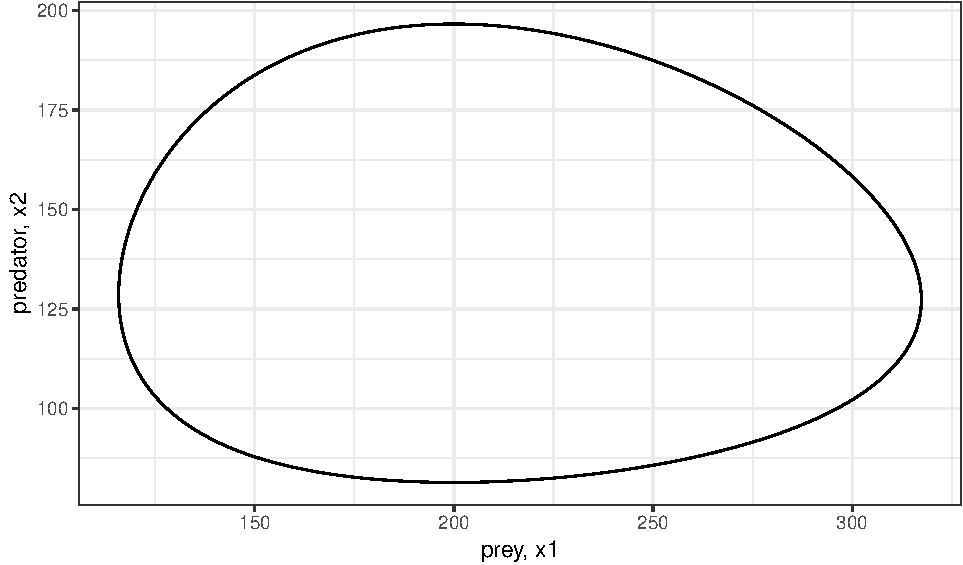
\includegraphics[width=0.85\linewidth]{_myDissertation_files/figure-latex/pp1Period-1} 

}

\caption{Phase space plot of two-species Lotka-Volterra predator-prey system over a single period (~11.145 time units.}\label{fig:pp1Period}
\end{figure}
\subsection{Concepts behind the
calculations}\label{concepts-behind-the-calculations}

Although the numerical steps for calculating the derivatives-based FI
are relatively straightforward, the concepts required to interpret the
measure in the context of multiple variables is more complex. Here, I
thoroughly discuss the concepts and assumptions behind FI calculation.
Below, steps do not represent steps within the calculation, they
represent the major concepts required

\subsubsection{\texorpdfstring{\textbf{Step 1. Probability of observing
the system in a particular state,
\(p(x)\)}}{Step 1. Probability of observing the system in a particular state, p(x)}}\label{step-1.-probability-of-observing-the-system-in-a-particular-state-px}
\begin{figure}

{\centering 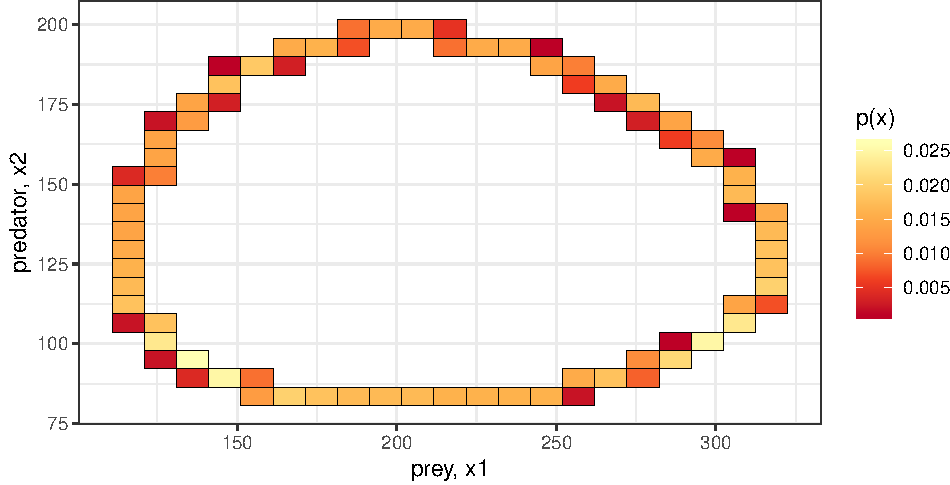
\includegraphics[width=0.85\linewidth]{_myDissertation_files/figure-latex/2D-hist-1} 

}

\caption{A 2-dimensional histogram of the probability of observing a system in a particular state, $p(x)$, of the 2-species Lotka-Volterra predator prey system over a single period (~11.145 time units).}\label{fig:2D-hist}
\end{figure}
Fisher Information (FI) is defined with respect to a probability
distribution. In the derivatives-based method, FI is calculated for a
probability of observing a system (as defined by one or more state
variables) in a particular state, \(p(x)\), over some period of time,
(\(0 to t_{end}\)). In other words \(p(x)\) is the probability that, at
a specific point in time (\(t_{obs}^*\)) we will observe the system in a
particular state, \(x^*\). The time at which we observe the system is a
random variable, \(t_{obs} ~ Uniform(0,t_{end})\). To be clear, the
study system is assumed to be deterministic and we assume no observation
error, however, the observed state of the system, \(x(T_{obs})\), is a
random variable because it is a function of the random observation time,
\(x^*= x(t_{obs}^*)\). The state of the model system, x, is defined in
two dimensions by the number of predators and the number of prey
\eqref{eq:predprey} and is easily visualized
\ref{fig:pp1Period}.Therefore, the probability of observing a particular
state is a two-dimensional joint distribution \ref{fig:2d-hist}.

A single state of the model system is defined by the number of predators
and prey at a given point in time such that for any given point in time
\(x(t)=[x_1 (t),x_2 (t)]\). At some random time between 0 and
\(t_{end}\) {[}\(T_{obs} ~ Uniform(0,t_{end})\){]} we can count the
number of predators and the number of prey to determine the state of the
model system. We must assume the system is deterministic and there is no
observation error. We can then calculate the probability of observing a
particular predator and prey abundance combination, \(p(x)\). Under
these assumptions, the only possible states of the system are defined by
the system's observed trajectory, the model parameters, and the initial
conditions. Therefore, the support of the probability distribution
\ref{fig:2D-hist} is the trajectory of the system.
\begin{figure}

{\centering 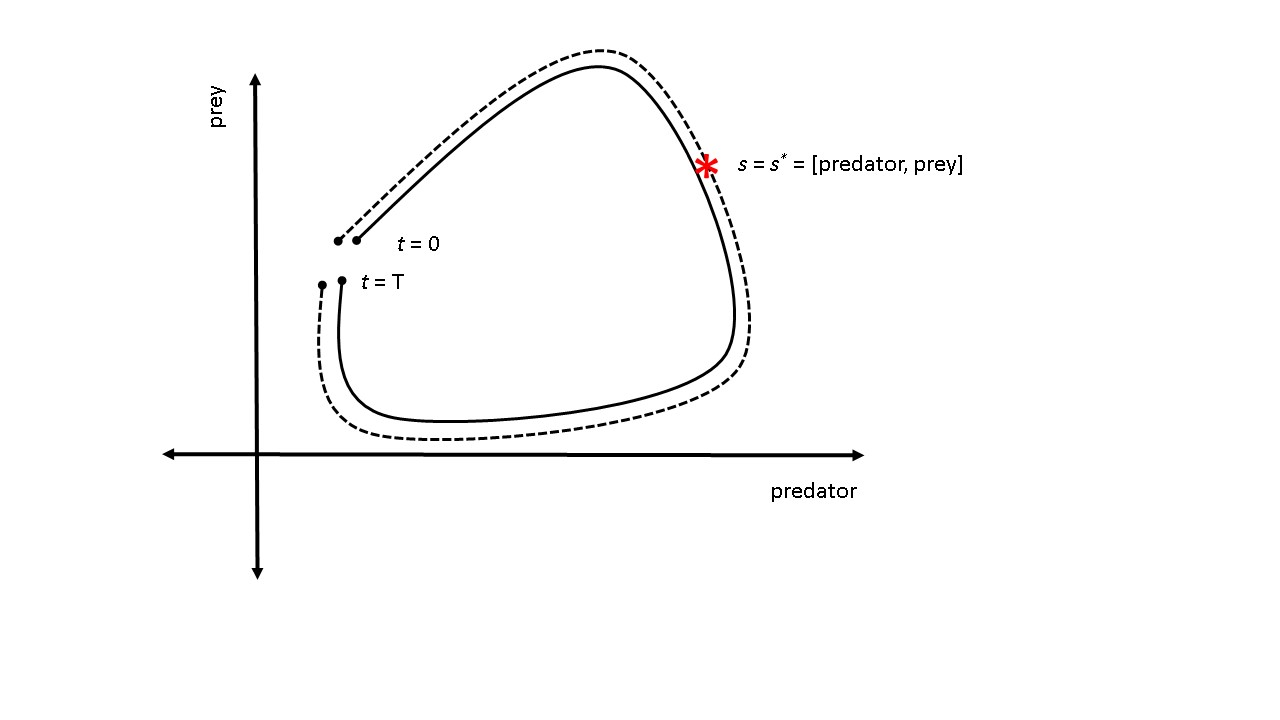
\includegraphics[width=0.95\linewidth]{./chapterFiles/fiGuide/figures/stringFig} 

}

\caption{A single cycle of a hypothetical two-species system over time period $t = 0$ to $t = T$. $s^*$ is the state of the system at some point in time. The dotted line represents the distance travelled by the system in phase space over its trajectory during time $(0, T)$.}\label{fig:stringFig}
\end{figure}
\subsubsection{\texorpdfstring{\textbf{Step 2.} Distance traveled by the
system,
\(s\)}{Step 2. Distance traveled by the system, s}}\label{step-2.-distance-traveled-by-the-system-s}

Distance traveled by the system, s. We can now move from an
n-dimensional representation of the probability distribution to a
one-dimensional representation. To better understand this, imagine
placing a string over the path of the entire trajectory from
\(0 to t_{end}\) \ref{fig:stringFig}. If we know the number of predators
and prey at a particular point in time \((t_{obs}^*)\) then we can mark
that location on the string (see asterisk in \ref{fig:stringFig}. Next,
imagine picking up the string and laying the string flat along a ruler.
The length, s, of the entire string measures the total distance traveled
by the system in phase space. The mark we made on the string (denoted
\(*\)) lies at a distance \(s^*\) between 0 and \(s\). We call this
length the distance traveled by the system, \(s^*\). In this context,
\(s^*\) in phase space represents a measure of cumulative change in
state. We note that the distance traveled in phase space increases
monotonically with time. If the system never revisits the same state
(i.e., the trajectory never overlaps or intersects itself), then every
unique system state (i.e., point on the trajectory) is mapped to a
unique value of distance traveled. Therefore, \(p(x)\) (n-dimensional)
is equivalent to the probability that the system is at distance s, i.e.,
\(p(x)=p(s)\), (where \(p(s)\) is one dimensional; Cabezas, Pawlowski,
Mayer, \& Hoagland (2005)). However, if the system revisits previous
states, then a unique system state may be mapped to different values of
distance traveled and the relationship between \(p(x)\) and \(p(s)\) is
not one-to-one. We calculated the distance traveled s of the model
system over a single cycle (11.145 time units; \ref{fig:distSpeedAccel}.
\begin{figure}

{\centering 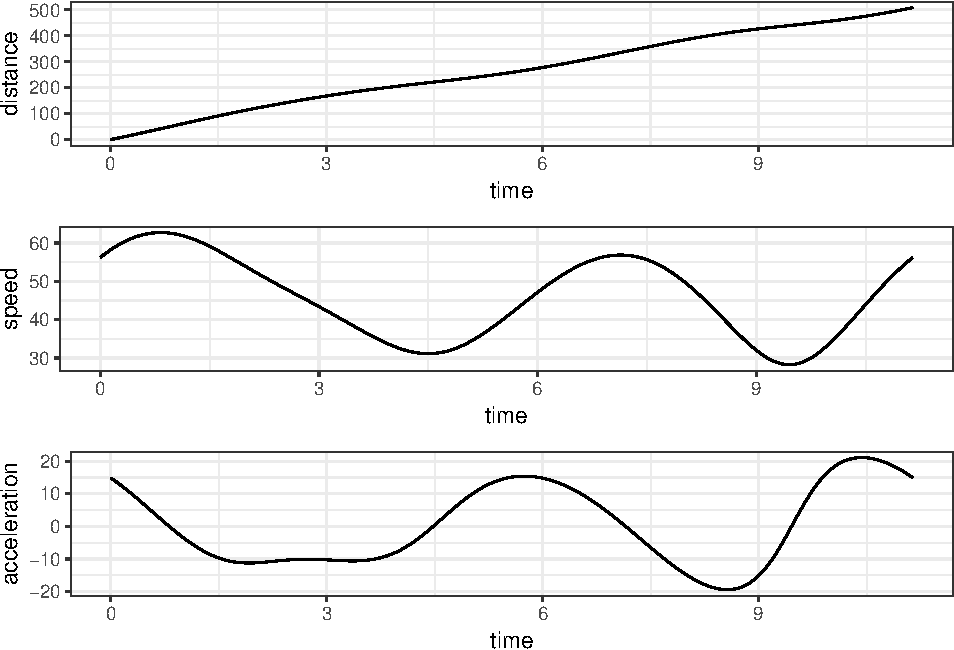
\includegraphics[width=0.85\linewidth]{_myDissertation_files/figure-latex/distSpeedAccel-1} 

}

\caption{From top to bottom, distance traveled in phase space, speed tangential to system trajectory, acceleration tangential to system trajectory.}\label{fig:distSpeedAccel}
\end{figure}
\subsubsection{\texorpdfstring{\textbf{Step 3.} \(p(s)\) as a function
of the rate of change of
\(s\)}{Step 3. p(s) as a function of the rate of change of s}}\label{step-3.-ps-as-a-function-of-the-rate-of-change-of-s}

In previous presentations of FI, the relationship between the state of
the system (n-dimensional) and the distance traveled (1-dimensional) was
not always emphasized (Cabezas \& Fath, 2002). Here we use x to denote
the state of the system and s to denote the distance traveled to
emphasize this distinction. If a system travels at a constant speed over
the entire time period, then the system is equally likely to be in any
state along the trajectory (\(s\) is linear and \(p(s)\) is uniform).
Referring to our model system, if the number of predators and prey are
linearly related, then the speed of the system is constant. For
non-linear systems, the distribution above the string will not be
uniform \ref{fig:stringFig}. Rather, it will change depending on the
amount of time the system spends in each state. It follows that \(p(s)\)
is proportional to the inverse of the rate of change of distance
traveled (i.e., the speed along the path in phase space).

We will now demonstrate this using our model system as an example.
Suppose the abundances of the predator and their prey in our model
system predictably operate at carrying capacity. Over a relatively short
period of time the prey abundance quickly declines after a severe
weather event (a pulse disturbance; (Bender et al. 1984), but quickly
recovers. Intuitively, the absolute rate of change at time points near
the disturbance will be larger than during time periods long before or
long after the disturbance. It is therefore more likely that the system
will be (observed) in a state where prey and predators are operating
approximately at carrying capacity than in a state with relatively low
prey abundance. Mathematically, the time, \(t*\), at which we calculate
the abundances of prey and predators is a uniform random variable, and
the distance traveled by the system, \(s^*\), is a function of time, is
differentiable, and monotonically increases. Therefore, the probability
density function of the distance traveled
\(p(s)=\frac{1}{T}\frac{1}{s'}\), where \(s'= \frac{ds}{dt}\) is the
speed of the system (the speed tangential to the trajectory; the first
derivative of the distance traveled; instantaneous rate of change of
\(s\)). We calculated the speed (the first derivative;
\ref{fig:distSpeedAccel} and acceleration (the second derivative;
\ref{fig:distSpeedAccel} of the distance traveled s by the model system
over a single cycle using function ode in package deSolve (Soetaert et
al. 2010) in Program R (R Core Team 2016).

\subsubsection{\texorpdfstring{\textbf{Step 4.} Calculate the
derivatives-based Fisher
Information}{Step 4. Calculate the derivatives-based Fisher Information}}\label{step-4.-calculate-the-derivatives-based-fisher-information}

Now that we understand how to calculate both the distance traveled,
\(s\), and its probability density, \(p(s)\), calculating the
derivatives-based FI is straightforward and computationally inexpensive
\eqref{eq:fiDerivs}. There are several comparable equations for
calculating the shift-invariant FI, and some may offer numerical
advantages over others. Equation \eqref{eq:fiAdapted} is the general form
and Equation \eqref{eq:fi73c} is the amplitude form for FI (in D. A. L.
Mayer et al. (2007), respectively). Although these formulations are
equivalent, \eqref{eq:fi73c} is most readily calculated when the
differential equations for the system are known, obviating any advantage
of a model-free metric.
\begin{equation}   
    I = \frac{1}{T} \int_0^T dt\left[\frac{s''^2}{s'^4}\right]^2 \\  
  \label{eq:fiDerivs}  
\end{equation}
\begin{equation} 
    I = \int \frac{ds}{p(s)}\left[\frac{dp(s)}{ds}\right]^2  \\
    \label{eq:fiAdapted}
\end{equation}
\begin{equation} 
    I = 4 \int ds\left[\frac{dq(s)}{ds}\right]^2 \\
\label{eq:fi73c}
\end{equation}
This article is interested in the Fisher Information calculated for a
distribution of distance traveled, \(s\), by the entire system. We
calculated the Fisher Information value using Equation \eqref{eq:fiDerivs}
over a single period of the model system (\eqref{eq:predprey}). We
calculated Fisher Information to be \(5.3\) x \(10^{-5}\) which is
consistent with the results of Mayer et al. (2007).

\section{Case Study}\label{case-study}

Mayer et al. (2007) calculated FI for a predator-prey system for several
discrete values of carrying capacity of prey. The results of this study
showed that FI was different for systems with different carrying
capacities. However, this study did not address the central question of
how FI changes during a regime shift. As an extension of the original
study, we simulate a regime shift by modeling a situation where carrying
capacity is abruptly decreased. To simulate an abrupt change in carrying
capacity, we assume carrying capacity is described by Eq. 6 where \(k1\)
is the initial carrying capacity, \(k2\) is the final carrying capacity,
\(t*\) is the time of the regime shift, and alpha is a parameter that
controls how quickly the regime shift occurs. The hyperbolic tangent
function simulates a smooth, continuous change in carrying capacity
while still allowing for the change to occur suddenly. To incorporate
the change in carrying capacity into the system differential equations
we define the rate of change of carrying capacity as given by
\eqref{eq:mayerCase}.\\
\begin{equation}  
  k(t) = k_1  - 0.5(k_1-k_2)(\tanh(\alpha (t-t^*))+1)     \\
  k'(t) = 0.5\alpha (k_1-k_2)(\tanh(\alpha(t-t^*))^2 +1)      \\ 
\label{eq:mayerCase}
\end{equation}
\begin{figure}

{\centering 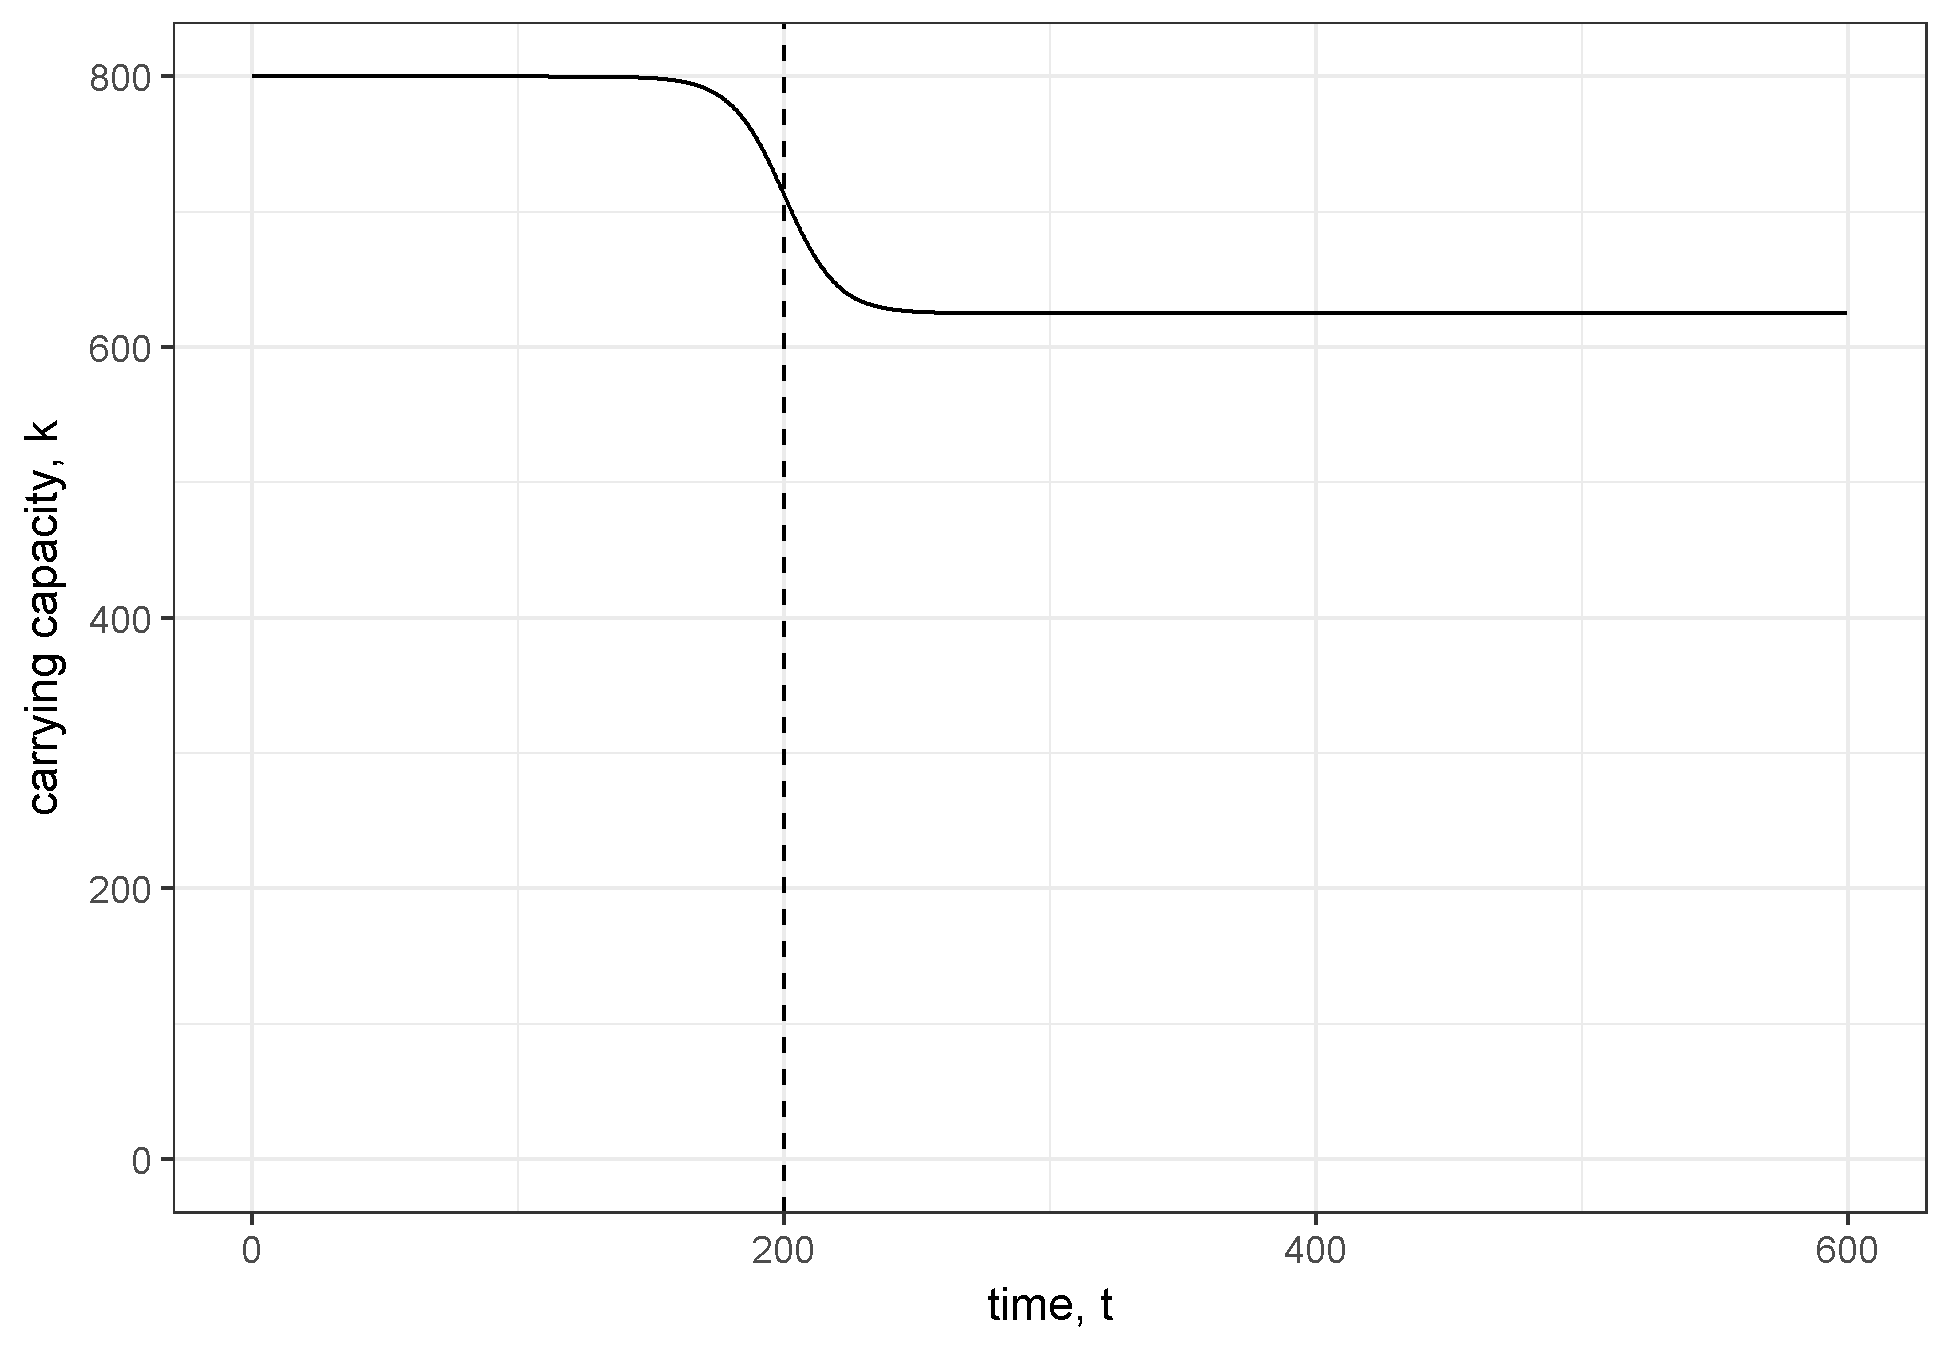
\includegraphics[width=0.85\linewidth]{./chapterFiles/fiGuide/figures/kByTime} 

}

\caption{Carrying capacity over time with a regime shift occuring around time 200.}\label{fig:kByTime}
\end{figure}\begin{figure}
{\centering 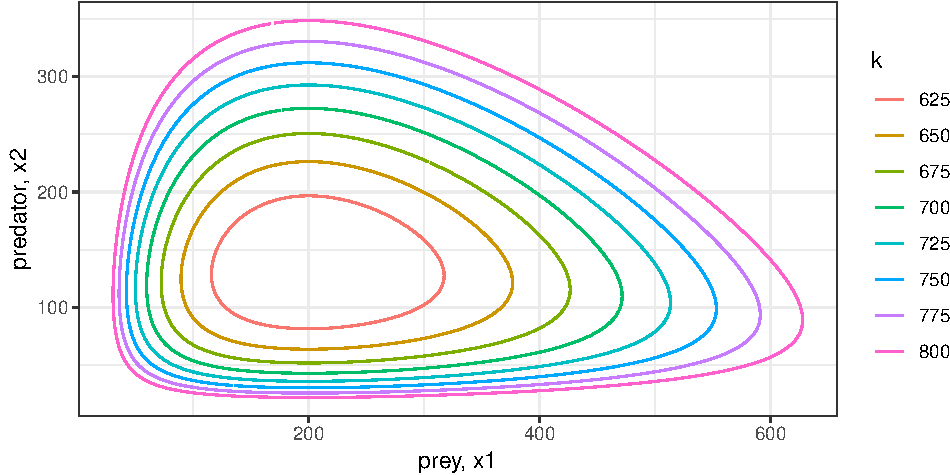
\includegraphics[width=0.85\linewidth]{_myDissertation_files/figure-latex/kTrajectories-1} 

}

\caption{Phase space plot of system trajectories for different values of k}\label{fig:kTrajectories}
\end{figure}
We assumed an initial carrying capacity of 800 and a final carrying
capacity of 625 which corresponds to the range of carrying capacities
explored by Mayer et al. (2007). We simulated a time series of 600 time
units with a regime change after 200 time units. We used an alpha value
of 0.05. The time series for carrying capacity is shown in
\ref{fig:kByTime} and the system trajectory in phase space is shown in
\ref{fig:kTrajectories}. The distance travelled in phase space (i.e.,
cumulative change in state) is shown in \ref{fig:distOverTime} and the
speed of the system (i.e., rate of change) is shown in
\ref{fig:dsdtOverTime}.
\begin{figure}

{\centering 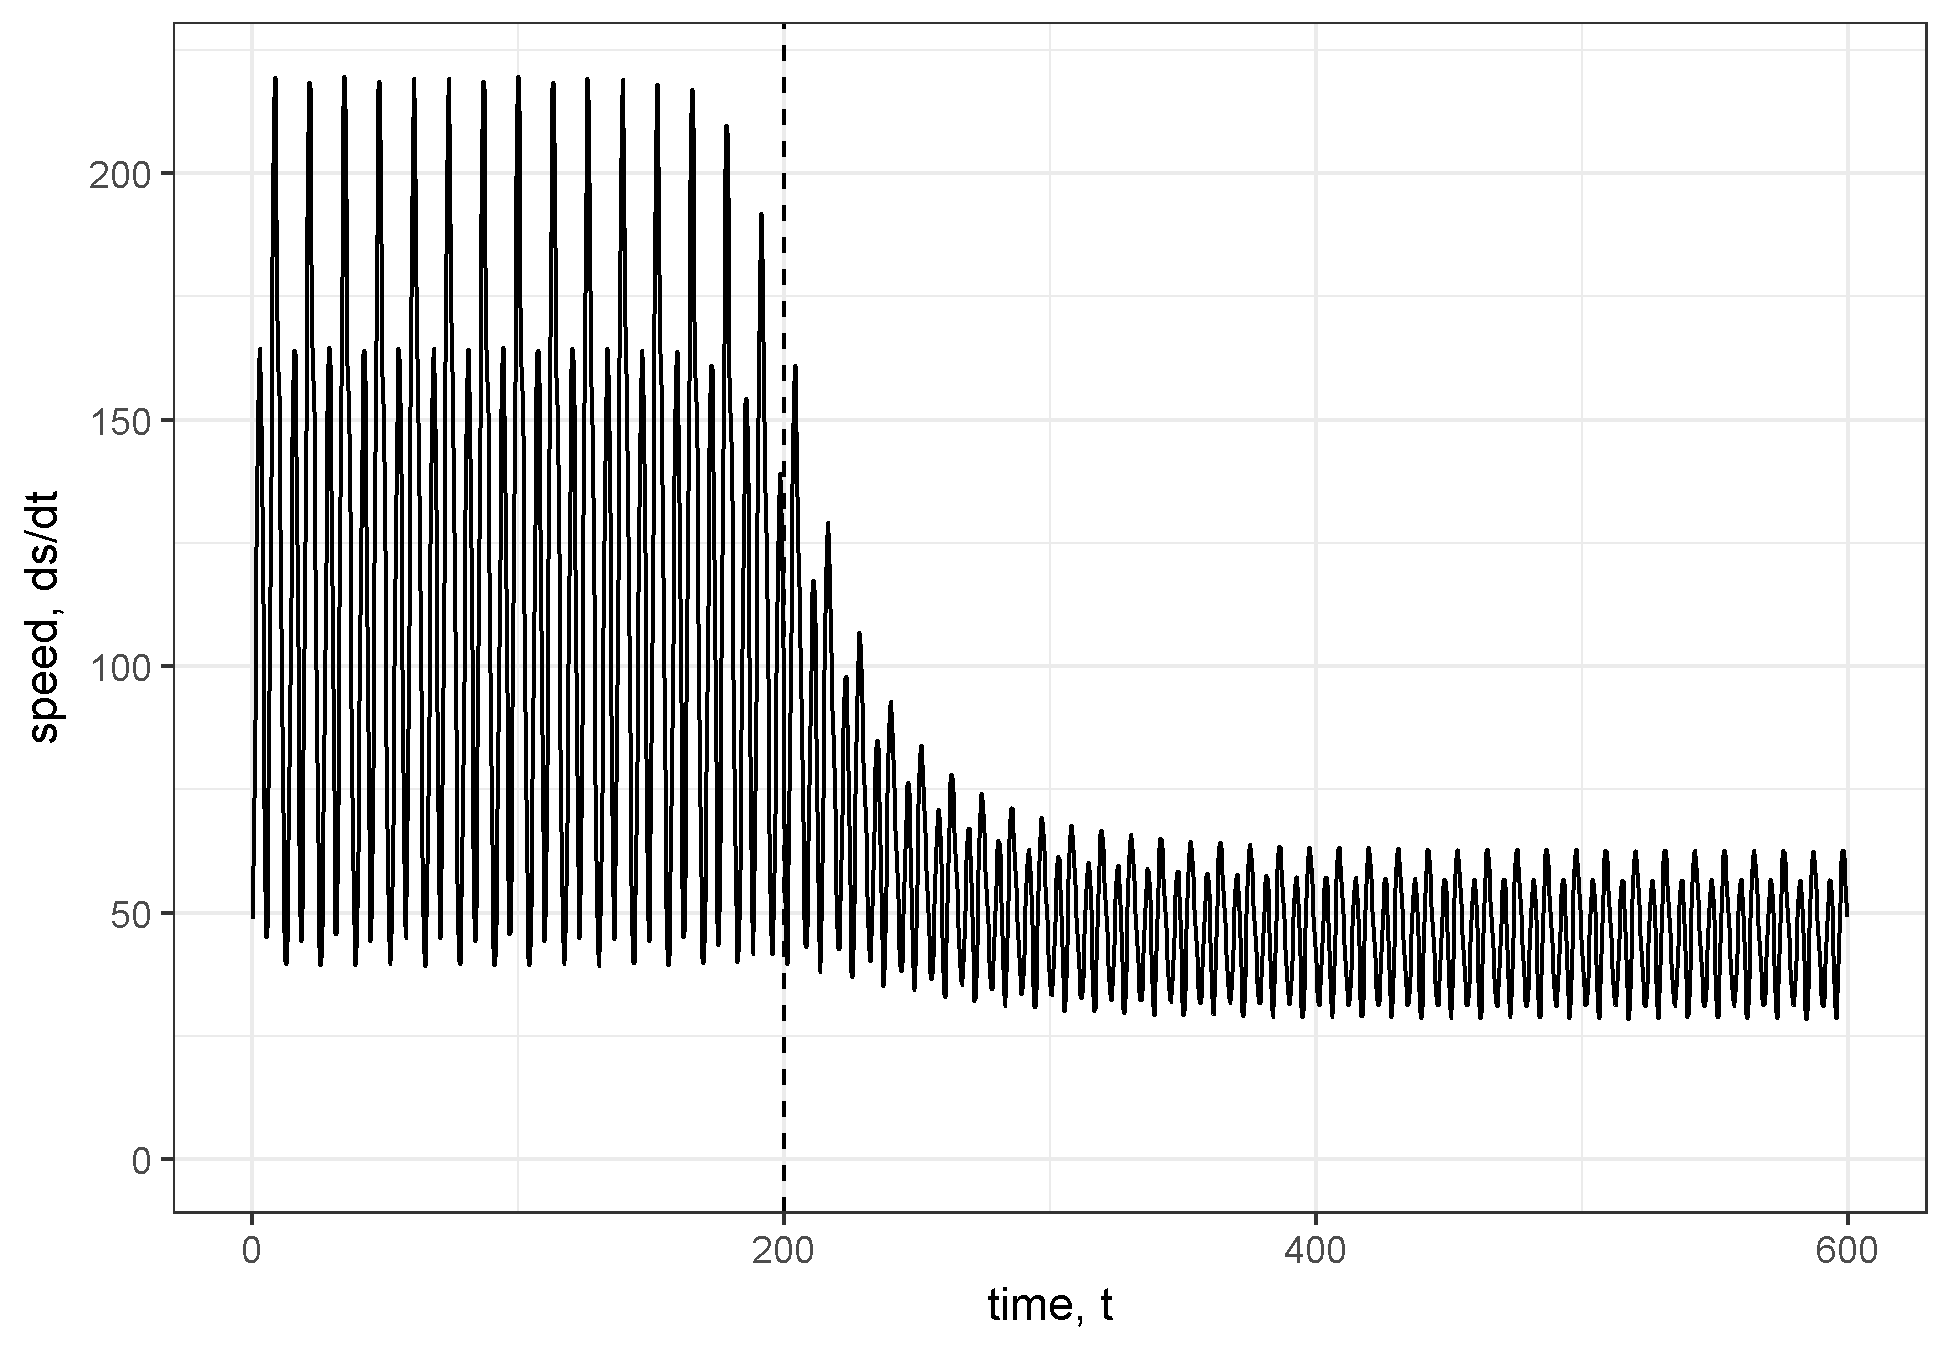
\includegraphics[width=0.85\linewidth]{./chapterFiles/fiGuide/figures/dsdtOverTime} 

}

\caption{Speed of the system (rate of change) in phase space. Dashed vertical line at time 200 indicates location of regime shift.}\label{fig:dsdtOverTime}
\end{figure}
We calculated FI for the distribution of distance travelled over a
series of non-overlapping time windows. Multiple sources suggest the
length of the time window should be equal to one system period such that
FI is constant for a periodic system (Cabezas \& Fath, 2002; D. A. L.
Mayer et al., 2007). However, the system period is different before,
during, and after the regime shift. Therefore, we performed two separate
calculations of FI using window sizes corresponding to the initial and
final period of the system (\(13.061\) and \(11.135\), respectively).
The change in FI over time is shown in \ref{fig:fiOverTime}.
\begin{figure}

{\centering \includegraphics[width=0.85\linewidth]{./chapterFiles/fiGuide/figures/fiOverTime} 

}

\caption{Fisher Information calculated for non-overlapping time windows. Two different window sizes were used as indicated by color. Dashed vertical line at time 200 indicates approximate location of regime shift.}\label{fig:fiOverTime}
\end{figure}
\section{Conclusions}\label{conclusions}

We simulated a regime shift caused by a change in carrying capacity
(\(K\)) within a simulated, two-species Lotka-Volterra system. I applied
the Fisher Information (FI) method for regime shift detection to the
simulated time series data. The predator-prey system was modeled as
deterministic and the time series data was free from measurement and
observation error. Despite this, the estimated FI had high variation
over time, and results were dependent on the size of the time window
used (winsize) in the calculation \ref{fig:fiOverTime}. The FI method
for regime shift detection is based on the cumulative change in the
state of the system (i.e., distance traveled in phase space) and the
rate of change of the system (i.e., speed tangential to trajectory in
phase space). The distance travelled metric, \(s\), and its speed,
\(dsdt\), appear better visual indicators of the regime shift than FI
{[}\ref{fig:distOverTime}; \ref{fig:dsdtOverTime}{]}.

In our explanation of the FI concept and calculation, I emphasize the
distinction between the \emph{state of the system} and the
\emph{distance traveled in phase space}. There are several reasons worth
emphasizing this. First, there may not always be a one-to-one
relationship between the probability of observing a system in a
particular state and the probability of observing a system at a
particular distance along the trajectory. In these situations the
interpretation of FI may be less clear than if a one-to-one relationship
existed. Second, this distinction facilitates the separation of the
dimensionality reduction step (calculating distance traveled in phase
space, \(s\)) from the subsequent steps related specifically to FI.
Third, the distinction suggests that the \textbf{value of FI as a regime
shift detection method is related to the rate of change of the system}
(i.e., velocity and acceleration tangential to system trajectory in
phase space). In particular, the distribution for which FI is calculated
is simply the distribution of the distance traveled in phase space, when
time is assumed to be uniformly distributed over a given interval.

Our results suggest that insights can be gained directly from the
calculation of distance traveled and associated rates of change.
Consequently, these insights preclude the need to calculate beyond Step
3 (described above). This result also supports the use of the distance
travelled metric, or the derivatives-based Fisher Information
\label{eq:fiDerivs}.

One remaining issue that is prevalent across ecological field studies is
the assumption that the system is observed without error. Although
ecological data rarely fulfill this assumption, this does not suggest
that FI is useless as a metric of system stability. The primary
difficulty with noisy data, especially with observations in integer form
(e.g.~count data), is that the denominator in can easily be zero for
some pair of observations, making FI an infinite value within windows
which contain two or more adjacent zero observations. One possible
solution is to smooth the multidimensional vector of observations prior
to calculating the derivatives, or to treat any sequential identical
value as missing, and simply use a larger time step for that portion of
the window calculation.

The utility of Fisher Information in ecological studies is also stunted
by its interpretability. This metric is unitless, making its values
relative only within-sample (e.g., within a single time series).
Further, interpreting the results within-sample is currently a
qualitative effort (B. D. Fath et al., 2003; Mantua, 2004). When the FI
of a system is increasing, the system is said to be moving toward a more
orderly state, and most presentations of FI posit sharp changes in FI,
regardless of the directionality of the change, may indicate a regime
shift (Cabezas \& Fath, 2002; Karunanithi et al., 2008; Spanbauer et
al., 2014). Due to the qualitative nature of these interpretations of
Fisher Information, intimate knowledge of the system in question and the
potential driver(s) of the observed regime shift are required to confirm
presence of a shift.

\section{Acknowledgements}\label{acknowledgements}

I thank T. Eason, H. Cabezas and B. Roy Frieden for early discussions
regarding Fisher Information.

\chapter{An application of Fisher Information to spatially-explicit
avian community data}\label{fisherSpatial}

Placeholder

\section{Introduction}\label{introduction-2}

\section{Data and methods}\label{data-and-methods}

\subsection{Data: North American breeding bird
communities}\label{data-north-american-breeding-bird-communities}

\subsection{Study area}\label{study-area}

\subsubsection{Focal military base}\label{focal-military-base}

\subsubsection{Spatial sampling grid}\label{spatial-sampling-grid}

\subsection{Calculating Fisher Information
(FI)}\label{calculating-fisher-information-fi}

\subsection{Interpreting and comparing Fisher Information across spatial
transects}\label{interpreting-and-comparing-fisher-information-across-spatial-transects}

\subsubsection{Interpreting Fisher Information
values}\label{interpreting-fisher-information-values}

\subsubsection{Interpolating results across spatial
transects}\label{interpolating-results-across-spatial-transects}

\subsubsection{Spatial correlation of Fisher
Information}\label{spatial-correlation-of-fisher-information}

\section{Results}\label{results-1}

\subsection{Fisher Information across spatial
transects}\label{fisher-information-across-spatial-transects}

\subsection{Spatial correlation of Fisher
Information}\label{spatial-correlation-of-fisher-information-1}

\section{Discussion}\label{discussion-1}

\subsection{Efficacy of Fisher Information as a spatial
RDM}\label{efficacy-of-fisher-information-as-a-spatial-rdm}

\chapter{\texorpdfstring{Velocity (\emph{v}): using rate-of-change of a
system's trajectory to identify abrupt
changes}{Velocity (v): using rate-of-change of a system's trajectory to identify abrupt changes}}\label{velocity}

Placeholder

\section{Introduction}\label{introduction-3}

\section{Data and methods}\label{data-and-methods-1}

\subsection{Theoretical system example: two-species time
series}\label{theoretical-system-example-two-species-time-series}

\subsection{\texorpdfstring{Steps for calculating system velocity,
\emph{v}}{Steps for calculating system velocity, v}}\label{steps-for-calculating-system-velocity-v}

\subsubsection{\texorpdfstring{Step 1:
\(\Delta x_i\)}{Step 1: \textbackslash{}Delta x\_i}}\label{step-1-delta-x_i}

\subsubsection{\texorpdfstring{Step 2:
\(\sqrt(\sum_i^N\Delta x_1^2)\)}{Step 2: \textbackslash{}sqrt(\textbackslash{}sum\_i\^{}N\textbackslash{}Delta x\_1\^{}2)}}\label{step-2-sqrtsum_indelta-x_12}

\subsubsection{\texorpdfstring{Step 3: Use Pythagorean theorem to
isolate
\(s\)}{Step 3: Use Pythagorean theorem to isolate s}}\label{step-3-use-pythagorean-theorem-to-isolate-s}

\subsubsection{\texorpdfstring{Step 4: Calculate velocity, \(v\) (or
\(\frac {\Delta s}{\Delta t}\))}{Step 4: Calculate velocity, v (or \textbackslash{}frac \{\textbackslash{}Delta s\}\{\textbackslash{}Delta t\})}}\label{step-4-calculate-velocity-v-or-frac-delta-sdelta-t}

\subsection{\texorpdfstring{Velocity \emph{v} performance under varying
mean and variance in the toy
system}{Velocity v performance under varying mean and variance in the toy system}}\label{velocity-v-performance-under-varying-mean-and-variance-in-the-toy-system}

\subsubsection{Varying post-shift mean}\label{varying-post-shift-mean}

\subsubsection{Varying post-shift
variance}\label{varying-post-shift-variance}

\subsubsection{\texorpdfstring{Smoothing the data prior to calculating
\emph{v}}{Smoothing the data prior to calculating v}}\label{smoothing-the-data-prior-to-calculating-v}

\subsection{Performance on empirical data: paleodiatom community
example}\label{performance-on-empirical-data-paleodiatom-community-example}

\section{Discussion}\label{discussion-2}

\section{Supplementary Materials}\label{supplementary-materials}

\chapter{Data Quality Impacts on Regime Detection
Measures}\label{resampling}

Placeholder

\section{Introduction}\label{introduction-4}

\section{Methods}\label{methods-1}

\subsection{Study system and data}\label{study-system-and-data}

\subsection{Regime detection measures}\label{regime-detection-measures}

\subsubsection{Variance index}\label{variance-index}

\subsubsection{Fisher Information}\label{fisher-information}

\subsubsection{\texorpdfstring{System velocity,
\(v\)}{System velocity, v}}\label{system-velocity-v}

\section{Results}\label{results-2}

\section{Discussion}\label{discussion-3}

\section{Ackowledgements}\label{ackowledgements}

\chapter{Discontinuity chapter under construction}\label{discontinuity}

\section{Introduction}\label{introduction-5}

\section{Data and Methods}\label{data-and-methods-2}

\section{Results}\label{results-3}

\section{Conclusions}\label{conclusions-1}

\chapter{Conclusions}\label{conclusions}

Placeholder

\section{Method mining regime detection
methods}\label{method-mining-regime-detection-methods}

\section{Ecological data are noisy}\label{ecological-data-are-noisy}

\section{Data collection and munging biases and limits
findings}\label{data-collection-and-munging-biases-and-limits-findings}

\section{Common Limitations of Regime Detection
Measures}\label{common-limitations-of-regime-detection-measures}

\section{Specific synthesis of chapter
results}\label{specific-synthesis-of-chapter-results}

\chapter*{Appendix A: R package
regimeDetectionMeasures}\label{regimeDetectionMeasures}
\addcontentsline{toc}{chapter}{Appendix A: R package
regimeDetectionMeasures}

Placeholder

\section{Measures/metrics calculated}\label{measuresmetrics-calculated}

\section{Example analysis}\label{example-analysis}

\chapter*{Appendix B: R package bbsRDM}\label{bbsRDM}
\addcontentsline{toc}{chapter}{Appendix B: R package bbsRDM}

Placeholder

\chapter*{References}\label{references}
\addcontentsline{toc}{chapter}{References}

Placeholder

\hypertarget{refs}{}
\hypertarget{ref-abadi2010assessment}{}
Abadi, F., Gimenez, O., Arlettaz, R., \& Schaub, M. (2010). An
assessment of integrated population models: Bias, accuracy, and
violation of the assumption of independence. \emph{Ecology},
\emph{91}(1), 7--14.

\hypertarget{ref-andersen_ecological_2009}{}
Andersen, T., Carstensen, J., Hern??ndez-Garc??a, E., \& Duarte, C. M.
(2009). Ecological thresholds and regime shifts: Approaches to
identification. \emph{Trends in Ecology \& Evolution}, \emph{24}(1),
49--57. \url{http://doi.org/10.1016/j.tree.2008.07.014}

\hypertarget{ref-beaugrand2004north}{}
Beaugrand, G. (2004). The north sea regime shift: Evidence, causes,
mechanisms and consequences. \emph{Progress in Oceanography},
\emph{60}(2-4), 245--262.

\hypertarget{ref-boettiger_quantifying_2012}{}
Boettiger, C., \& Hastings, A. (2012). Quantifying limits to detection
of early warning for critical transitions. \emph{Journal of the Royal
Society Interface}, \emph{9}, 2527--39.

\hypertarget{ref-cabezas_towards_2002}{}
Cabezas, H., \& Fath, B. D. (2002). Towards a theory of sustainable
systems. \emph{Fluid Phase Equilibria}, \emph{194}(Supplement C), 3--14.
\url{http://doi.org/10.1016/S0378-3812(01)00677-X}

\hypertarget{ref-cabezas_simulated_2005}{}
Cabezas, H., Pawlowski, C. W., Mayer, A. L., \& Hoagland, N. T. (2005).
Simulated experiments with complex sustainable systems: Ecology and
technology. \emph{Resources, Conservation and Recycling}, \emph{44}(3),
279--291. Retrieved from
\url{http://www.sciencedirect.com/science/article/pii/S092134490500025X}

\hypertarget{ref-dakos_methods_2012}{}
Dakos, V., Carpenter, S. R., Brock, W. A., Ellison, A. M., Guttal, V.,
Ives, A. R., \ldots{} Nes, E. H. van. (2012). Methods for detecting
early warnings of critical transitions in time series illustrated using
simulated ecological data. \emph{PloS One}, \emph{7}(7), e41010.

\hypertarget{ref-fath_exergy_2004}{}
Fath, B. D., \& Cabezas, H. (2004). Exergy and Fisher Information as
ecological indices. \emph{Ecological Modelling}, \emph{174}(1), 25--35.
\url{http://doi.org/10.1016/j.ecolmodel.2003.12.045}

\hypertarget{ref-fath_regime_2003}{}
Fath, B. D., Cabezas, H., \& Pawlowski, C. W. (2003). Regime changes in
ecological systems: An information theory approach. \emph{Journal of
Theoretical Biology}, \emph{222}(4), 517--530.
\url{http://doi.org/10.1016/S0022-5193(03)00067-5}

\hypertarget{ref-fisher_mathematical_1922}{}
Fisher, R. A. (1922). On the Mathematical Foundations of Theoretical
Statistics. \emph{Philosophical Transactions of the Royal Society of
London. Series A, Containing Papers of a Mathematical or Physical
Character}, \emph{222}, 309--368. Retrieved from
\url{http://www.jstor.org/stable/91208}

\hypertarget{ref-frieden_physics_1998}{}
Frieden, B. R. (1998). \emph{Physics from Fisher information: A
unification.} New York, NY: Cambridge University Press.

\hypertarget{ref-frieden_exploratory_2007}{}
Frieden, B. R., \& Gatenby, R. (Eds.). (2007). \emph{Exploratory Data
Analysis Using Fisher Information}. Springer. Retrieved from
\url{http://www.springer.com/us/book/9781846285066}

\hypertarget{ref-hastings_regime_2010}{}
Hastings, A., \& Wysham, D. B. (2010). Regime shifts in ecological
systems can occur with no warning. \emph{Ecology Letters}, \emph{13}(4),
464--472. \url{http://doi.org/10.1111/j.1461-0248.2010.01439.x}

\hypertarget{ref-hefley2013statistical}{}
Hefley, T. J., Tyre, A. J., \& Blankenship, E. E. (2013). Statistical
indicators and state--space population models predict extinction in a
population of bobwhite quail. \emph{Theoretical Ecology}, \emph{6}(3),
319--331.

\hypertarget{ref-jorgensen_towards_2004}{}
Jorgensen, S. E., \& Svirezhev, Y. M. (2004). \emph{Towards a
Thermodynamic Theory for Ecological Systems}. Elsevier.

\hypertarget{ref-karunanithi_detection_2008}{}
Karunanithi, A. T., Cabezas, H., Frieden, B. R., \& Pawlowski, C. W.
(2008). Detection and assessment of ecosystem regime shifts from fisher
information. \emph{Ecology and Society}, \emph{13}(1).

\hypertarget{ref-mantua_methods_2004}{}
Mantua, N. (2004). Methods for detecting regime shifts in large marine
ecosystems: A review with approaches applied to North Pacific data.
\emph{Progress in Oceanography}, \emph{60}(2), 165--182.
\url{http://doi.org/10.1016/j.pocean.2004.02.016}

\hypertarget{ref-mayer_applications_2007}{}
Mayer, D. A. L., Pawlowski, D. C., Fath, P. B. D., \& Cabezas, D. H.
(2007). Applications of Fisher Information to the Management of
Sustainable Environmental Systems. In B. R. F. B. MS \& R. A. G. B. MD
(Eds.), \emph{Exploratory Data Analysis Using Fisher Information} (pp.
217--244). Springer London.
\url{http://doi.org/10.1007/978-1-84628-777-0_7}

\hypertarget{ref-perretti_model-free_2013}{}
Perretti, C. T., Munch, S. B., \& Sugihara, G. (2013). Model-free
forecasting outperforms the correct mechanistic model for simulated and
experimental data. \emph{Proceedings of the National Academy of
Sciences}, \emph{110}(13), 5253--5257.

\hypertarget{ref-petersen2008regime}{}
Petersen, J. K., Hansen, J. W., Laursen, M. B., Clausen, P., Carstensen,
J., \& Conley, D. J. (2008). Regime shift in a coastal marine ecosystem.
\emph{Ecological Applications}, \emph{18}(2), 497--510.

\hypertarget{ref-rodionov_application_2005}{}
Rodionov, S., \& Overland, J. E. (2005). Application of a sequential
regime shift detection method to the Bering Sea ecosystem. \emph{ICES
Journal of Marine Science}, \emph{62}(3), 328--332.
\url{http://doi.org/10.1016/j.icesjms.2005.01.013}

\hypertarget{ref-roy_frieden_physics_1998}{}
Roy Frieden, B. (1998). \emph{Physics from Fisher information}.
Cambridge: Cambridge University Press.

\hypertarget{ref-scheffer_catastrophic_2001}{}
Scheffer, M., Carpenter, S., Foley, J. A., Folke, C., \& Walker, B.
(2001). Catastrophic shifts in ecosystems. \emph{Nature},
\emph{413}(6856), 591--596.

\hypertarget{ref-spanbauer_prolonged_2014}{}
Spanbauer, T. L., Allen, C. R., Angeler, D. G., Eason, T., Fritz, S. C.,
Garmestani, A. S., \ldots{} Stone, J. R. (2014). Prolonged instability
prior to a regime shift. \emph{PLoS One}, \emph{9}(10), e108936.

\hypertarget{ref-walther_ecological_2002}{}
Walther, G.-R., Post, E., Convey, P., Menzel, A., Parmesan, C., Beebee,
T. J., \ldots{} Bairlein, F. (2002). Ecological responses to recent
climate change. \emph{Nature}, \emph{416}(6879), 389.


\end{document}
